\subsection{Historique}

\begin{frame}{Où trouver les versions des supports de cours ?}

Les supports de cours imprimables au format élecronique sont accessibles sur Plei@d (\url{http://idf.pleiad.net/}). Vous devez avoir un accès à Plei@d et aux supports de l'UE dès votre inscription finalisée. \\

\bigskip

TP : Comment fonctionnent les salles de TP ? Quels sont mes login et mot de passe pour me connecter (\`a r\'ecup\'erer avant le premier TP) ? ... etc ?
\url{http://ressources-informatiques.cnam.fr/}

\end{frame}

\begin{frame}[allowframebreaks]{Historique}

\begin{description}
\item[1969]  GML : Langage permettant de dissocier contenu des sp\'ecificit\'es techniques des imprimantes;
\item[1986] SGML (ISO, organisation internationale de normalisation) : Standard Generalized Markup Language. Successeur de GML. \prof{pour spécification de divers documents}
\item[1991] HTML : Application de SGML pour le web. "Mauvaise" utilisation de SGML.
\end{description}

\prof{SGML : Standard Generalized Markup Language \\
ISO : Organisation internationale de normalisation (ISO) \\
HTML : Hypertext Markup Language - application de SGML pour le web \\
1998: proposition XML 1.0 par la W3C\\
XML : simplification de SGML pour le web. SGML aurait pu suffire mais on a cr\'e\'e une norme ``\`a la internet''
}

\framebreak

La gestion des donn\'ees du web a tout d'abord \'et\'e fond\'ee sur HTML, qui contient \`a la fois contenu et pr\'esentation ``m\'elang\'es''
\begin{itemize}
\item HTML est appropri\'e pour les humains : permet des sorties sophistiqu\'ees et les interactions avec texte et images,
\item HTML devient limit\'e lorsque il s'agit d'exploiter automatiquement les donn\'ees par les logiciels. 
\end{itemize}

\begin{block}{}
N\'ecessit\'e d'un format de publication dissociant contenu et pr\'esentation, de fa\c{c}on \`a rendre le contenu exploitable par un programme.
\end{block}

\framebreak

Les donn\'ees (\'eventuellement volumineuses) circulent :
\begin{itemize}
\item en interne dans l'entreprise,
\item vers l'ext\'erieur.
\end{itemize}
entre plate-formes d'exploitation \'eventuellement diff\'erentes.

\begin{block}{}
N\'ecessit\'e d'un format d'\'echange de contenu ``souple'' s'auto-d\'ecrivant (encodage et contenu) ind\'ependant de toute plate-forme.
\end{block}

\prof{API : Application Programming Interface. C'est un ensemble de fonctions, proc\'edures ou classes mises \`a disposition des programmes informatiques par une biblioth\`eque logicielle, un syst\`eme d'exploitation ou un service}

\framebreak

En repartant de SGML, cr\'eation de XML qui est une application de SGML pour le web mais pas que !\\

Valid\'e par le W3C (World Wide Web Consortium).

\prof{Extrait site W3C : The World Wide Web Consortium (W3C) is an international community that develops standards to ensure the long-term growth of the Web}

\framebreak

XML d\'ecrit du contenu, facilite la communication machine-\`a-machine et l'\'echange des donn\'ees
\begin{itemize}
\item XML est un format de donn\'ees g\'en\'erique permettant de manipuler donn\'ees structur\'ees et semi-structur\'ees,
\item XML facilite l'int\'egration des donn\'ees \`a partir du moment o\`u source et destination partagent maintenant un language commun,
\item XML vient avec toute une panoplie de logiciels, APIs, outils, applications.
\end{itemize}

\end{frame}

\subsection{Introduction au mod\`ele de donn\'ees}

\begin{frame}{Un mod\`ele pour les donn\'ees semi-structur\'ees}
Id\'ees de base :

\begin{itemize}
\item Mod\`ele de donn\'ees, fond\'e sur les arbres (plus généralement les graphes),\prof{en tenant compte des références} permettant de repr\'esenter des donn\'ees r\'eguli\`eres et des donn\'ees irr\'eguli\`eres (mais pas trop). \textbf{$\rightarrow$ donn\'ees semi-structur\'ees}.
\item Typage souple.
\item Repr\'esentable en \textit{serialized form} afin d'\^etre \textbf{\'echang\'e entre applications}.
\end{itemize}

\end{frame}



\begin{frame}{Document XML}

Un document XML est un arbre pour lequel :
\begin{itemize}
\item les n{\oe}uds sont \'etiquet\'es,
\item le nombre de fils d'un n{\oe}ud n'est pas limit\'e,
\item les fils d'un n{\oe}ud sont ordonn\'es.
\end{itemize}

\end{frame}


\begin{frame}{Document XML}
Un document XML repr\'esente un arbre.
\begin{center}
\small
\smallskip
\tikzstyle{lien}=[-,>=stealth,rounded corners=5pt] 
%\tikzset{internal/.style={draw,rounded corners=1mm}}
%\tikzset{leaf/.style={draw,thick}, leaf/.default={green}}
\tikzset{internal/.style={rounded corners=1mm},text centered}
\tikzset{leaf/.style={}, leaf/.default={green},text centered}
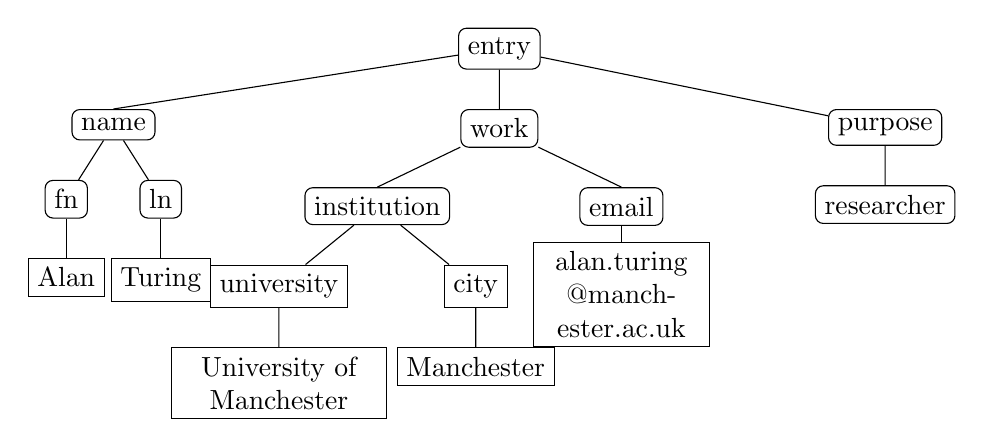
\begin{tikzpicture} [level distance=0.5cm, anchor=north, growth parent anchor=south,sibling distance=4.9cm]%[scale=0.5,level distance=3cm, sibling distance=6cm]
  \node [internal] {entry}
  child { [sibling distance=1.2cm] 
    node [internal]{name} 
    child { node [internal]{fn} child{ node [leaf]{Alan}}  }
    child { node [internal]{ln} child{ node [leaf]{Turing}} } 
  }
  child { [sibling distance=3.1cm]  
    node [internal]{work} 
   child { [sibling distance=2.5cm]  node [internal]{institution} 
      child{ node [leaf]{university}  child{ node [leaf,text width=2.5cm]{University of Manchester}  } } 
      child{ node [leaf]{city}  child{ node [leaf]{Manchester}  } } }
    child { [level distance=0.2cm] node [internal]{email} child{ node [leaf,text width=2cm]{alan.turing @manchester.ac.uk}} } 
  }
  child { 
    node [internal]{purpose} 
    child { node [internal]{researcher} }
 }
; 
\end{tikzpicture}
\end{center}
\end{frame}


\begin{frame}[containsverbatim]{Document XML}

\begin{tabular}{ p{5cm} | p{5cm}  }
Les composants fondamentaux d'un document XML sont l'\textit{\'el\'ement} et le \textit{texte}.&Sous forme d'arbre :\\

\begin{verbatim}
<elt_name> 
  Textual content 
</elt_name>
\end{verbatim}
&
\begin{center}
{
\tikzstyle{lien}=[-,>=stealth,rounded corners=5pt] 
%\tikzset{internal/.style={draw,rounded corners=1mm}}
%\tikzset{leaf/.style={draw,thick}, leaf/.default={green}}
\tikzset{internal/.style={draw,rounded corners=1mm},text centered}
\tikzset{leaf/.style={draw}, leaf/.default={green},text centered}
\begin{tikzpicture} [level distance=0.5cm, anchor=north, growth parent anchor=south,sibling distance=4.9cm]%[scale=0.5,level distance=3cm, sibling distance=6cm]
  \node [internal, text width=2cm] {\textbf{Element} \verb?elt_name?}
  child { node[leaf, text width=3cm]{\textbf{Text} \mbox{\verb?Textual\ content? }} }
; 
\end{tikzpicture}
}
\end{center}
\\
\end{tabular}
\end{frame}



\begin{frame}{Document XML}
Un document XML repr\'esente un arbre.
\begin{center}
\small
\smallskip
\tikzstyle{lien}=[-,>=stealth,rounded corners=5pt] 
%\tikzset{internal/.style={draw,rounded corners=1mm}}
%\tikzset{leaf/.style={draw,thick}, leaf/.default={green}}
\tikzset{internal/.style={draw,rounded corners=1mm},text centered}
\tikzset{leaf/.style={draw}, leaf/.default={green},text centered}
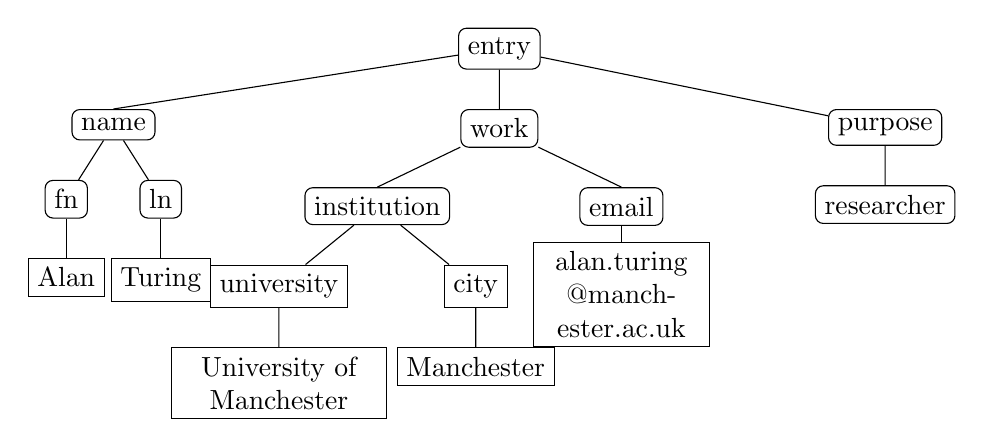
\begin{tikzpicture} [level distance=0.5cm, anchor=north, growth parent anchor=south,sibling distance=4.9cm]%[scale=0.5,level distance=3cm, sibling distance=6cm]
  \node [internal] {entry}
  child { [sibling distance=1.2cm] 
    node [internal]{name} 
    child { node [internal]{fn} child{ node [leaf]{Alan}}  }
    child { node [internal]{ln} child{ node [leaf]{Turing}} } 
  }
  child { [sibling distance=3.1cm]  
    node [internal]{work} 
   child { [sibling distance=2.5cm]  node [internal]{institution} 
      child{ node [leaf]{university}  child{ node [leaf,text width=2.5cm]{University of Manchester}  } } 
      child{ node [leaf]{city}  child{ node [leaf]{Manchester}  } } }
    child { [level distance=0.2cm] node [internal]{email} child{ node [leaf,text width=2cm]{alan.turing @manchester.ac.uk}} } 
  }
  child { 
    node [internal]{purpose} 
    child { node [internal]{researcher} }
 }
; 
\end{tikzpicture}
\end{center}
\end{frame}


\begin{frame}[containsverbatim]{Forme s\'erialis\'ee}
Avec indentation pour am\'eliorer la lisibilit\'e :
\begin{lstlisting}
<entry> 
 <name>
  <fn>Alan</fn>
  <ln>Turing</ln>
 </name>
 <work>
  <institution>
   <university>University of Manchester<university>
   <city>Manchester</city>
  </institution>
  <email>alan.turing@manchester.ac.uk</email>
 </work>
 <purpose>researcher</purpose>
</entry>
\end{lstlisting}
\end{frame}

\begin{frame}[containsverbatim]{Forme s\'erialis\'ee}
Un document peut \^etre s\'erialis\'e (obtenu par parcours d'arbre pr\'efixe\prof{Racine puis les fils}) :  
\begin{lstlisting}[basicstyle=\small,showstringspaces=false,frame=trBL,language=XML,escapechar=?,breaklines=true,columns=fullflexible,breakautoindent=false,breakindent=0pt]
<entry><name><fn>Alan</fn><ln>Turing</ln></name><work><institution><university>University of Manchester<university><city>Manchester</city></institution><email>alan.turing@manchester.ac.uk</email></work><purpose>researcher</purpose></entry>
\end{lstlisting}
\end{frame}

\begin{frame}{Mais attention !}
XML d\'efinit \textbf{juste une syntaxe} : aucune s'\'emantique n'est \emph{a priori} associ\'ee aux \'etiquettes.
\end{frame}

\begin{frame}[containsverbatim, allowframebreaks]{Document XML}
Les programmes peuvent difficilement interpr\'eter un contenu non structur\'e : 

\bigskip

\texttt{\footnotesize The book ``Fundations of Databases'', written by Serge Abiteboul, 
Rick Hull and Victor Vianu, published in 1995 by Addison-Wesley 
}

\framebreak

XML fournit un moyen de structurer ce contenu :
\begin{lstlisting}[basicstyle=\footnotesize,showstringspaces=false,frame=trBL,language=XML,escapechar=?,breaklines=false,columns=fullflexible]
<bibliography> 
  <book> 
    <title> Foundations of Databases </title> 
    <author> Serge Abiteboul </author> 
    <author> Rick Hull </author> 
    <author> Victor Vianu </author> 
    <publisher> Addison-Wesley </publisher> 
    <year> 1995 </year> 
  </book> 
  <book>...</book> 
</bibliography> 
\end{lstlisting} 
Un programme peut alors acc\'eder \`a l'arbre XML, en extraire des parties, renommer des \'etiquettes, r\'e-organiser le contenu de l'arbre ou transformer l'arbre en un document ayant une structure compl\`etement diff\'erente, etc.

\end{frame}


\begin{frame}[containsverbatim]{Processeur XML et forme s\'erialis\'ee}

\begin{itemize}
\item La forme s\'erialis\'ee est une repr\'esentation textuelle lin\'eaire d'un arbre satisfaisant une syntaxe.
\item Il existe un mod\`ele orient\'e-objet permettant de repr\'esenter des donn\'ees XML sous forme d'arbre : Document Object Model (W3C). Les applications ``travaillent'' avec ce genre de repr\'esentations sous forme d'arbre.
\end{itemize}

Comportement typique d'une application acceptant des documents XML en entr\'ee :

\begin{center}
\begin{tikzpicture}[node distance=1.3cm,>=stealth',bend angle=45,auto]
\footnotesize
  \tikzstyle{emptyStyle}=[text width=1cm]
  \tikzstyle{parser}=[rounded corners=3mm,thick,draw=blue!75,fill=blue!20,minimum size=6mm,text centered]
  \tikzstyle{appli}=[rounded corners=1mm,thick,draw=red!75,fill=red!20,text centered,text width=2cm]
  \tikzstyle{every label}=[red]

  \begin{scope}
    \node[emptyStyle](sf1) at (0,0) {\it Forme s\'erialis\'ee};
    \node[parser, right= 0.8cm of sf1](parser) {Processeur};
    \node[appli, right= 0cm of parser](appli)  {Application \linebreak {\it Forme d'arbre}};
    \node[parser,right= 0cm of appli](serial) {Serialiseur};
    \node[emptyStyle,right= 0.8cm of serial](sf2) {\it Forme s\'erialis\'ee};
    \draw[->,>=latex] (sf1) -- (parser);
    \draw[->,>=latex] (serial) -- (sf2);
\end{scope}

  \begin{pgfonlayer}{background}
    \filldraw [line width=4mm,join=round,black!20]
      (parser.north  -| parser.west)  rectangle (serial.south  -| serial.east);
 \end{pgfonlayer}
\end{tikzpicture}
\end{center}

\prof{Le \textbf{processeur}, validant ou non, parse le document (le valide si le processeur est validant -et modifie \'eventuellement le doc avec les informations du sch\'ema si le sch\'ema contient par exemple des valeurs par d\'efaut-, sinon ne le valide pas) et le met \`a disposition de l'application sous forme d'arbre.
%http://www.w3.org/TR/REC-xml/#dt-xml-proc
Definition: A software module called an XML processor is used to read XML documents and provide access to their content and structure. Definition: It is assumed that an XML processor is doing its work on behalf of another module, called the application. (Extensible Markup Language (XML) 1.0 (Fifth Edition)
W3C Recommendation 26 November 2008). Processeur donne accès aux données (effectue les remplacement si besoins en fonction de la DTD s'il est validant). Il peut être non validant et dans ce cas ne pas tenir compte de ce qui est déclaré dans le DTD, par exemple les valeurs par défaut.
Le \textbf{parser}, validant ou non, ne fait que vérifier la syntaxe ?
}

\end{frame}



\begin{frame}[containsverbatim]{Le formalisme XML, pourquoi ?}

\begin{description}
\item[Format]  convention utilis\'ee pour repr\'esenter des donn\'ees.
\item[Ouvert] sp\'ecification publiquement accessible.
\item[Normalis\'e] valid\'e par un organisme de normalisation (ici, le W3C).
\end{description}

\begin{center}
\begin{tikzpicture}[node distance=1.3cm,>=stealth',bend angle=45,auto]
\footnotesize
  \tikzstyle{emptyStyle}=[text width=0.7cm]
  \tikzstyle{parser}=[rounded corners=3mm,thick,draw=blue!75,fill=blue!20,minimum size=6mm,text centered]
  \tikzstyle{appli}=[rounded corners=1mm,thick,draw=red!75,fill=red!20,text centered,text width=2cm]
  \tikzstyle{every label}=[black]

  \begin{scope}
    \node[emptyStyle](sf1) at (0,0) {\it Forme s\'erialis\'ee};
    \node[parser, right= 0.8cm of sf1](parser) {Processeur};
    \node[appli, right= 0cm of parser, label= Application 1](appli)  {Application \linebreak {\it Forme d'arbre}};
    \node[parser,right= 0cm of appli](serial) {Serialiseur};
    \node[emptyStyle,right= 0.8cm of serial](sf2) {\it Forme s\'erialis\'ee};
    \draw[->,>=latex] (sf1) -- (parser);
    \draw[->,>=latex] (serial) -- (sf2);
    \node[parser, below= 2cm of appli](parser2) {Processeur};
    \node[appli, right= 0cm of parser2, label= Application 2](appli2)  {Application \linebreak {\it Forme d'arbre}};
    \node[parser,right= 0cm of appli2](serial2) {Serialiseur};
    \node[emptyStyle,right= 0.8cm of serial2](sf3) {\it Forme s\'erialis\'ee};
    \draw[->,>=latex] (sf2) -- ++ (parser2);
    \draw[->,>=latex] (serial2) -- (sf3);
\end{scope}

  \begin{pgfonlayer}{background}
    \filldraw [line width=4mm,join=round,black!20]
      (parser.north  -| parser.west)  rectangle (serial.south  -| serial.east);
\end{pgfonlayer}

  \begin{pgfonlayer}{background}
    \filldraw [line width=4mm,join=round,black!20]
     (parser2.north  -| parser2.west)  rectangle (serial2.south  -| serial2.east);
 \end{pgfonlayer}

\end{tikzpicture}
\end{center}

\begin{block}{Objectif}
\textit{Interop\'erabilit\'e} des applications.
\end{block}

\end{frame}


\begin{frame}[containsverbatim]{Sch\'ema}

Il est possible d'associer un sch\'ema \`a un ou plusieurs documents XML.\\
Un sch\'ema d\'efinit un ensemble de contraintes \underline{syntaxiques} que des documents doivent satisfaire.

\begin{footnotesize}

\lstinputlisting[firstline=2,basicstyle=\tiny]{codes/exemple_persons.xml}

\end{footnotesize}

\begin{block}{Toujours dans le m\^eme objectif}
\textit{Interop\'erabilit\'e} des applications.
\end{block}

\prof{Bien form\'e si satisfait la syntaxe XML. Valide si satisfait le sch\'ema qui lui est associ\'e.
Validation effectu\'ee sur http://www.validome.org/xml/validate/
}

\end{frame}


\begin{frame}[containsverbatim]{Et la s\'emantique ?}

Que d\'ecrivent les documents XML suivants ?
\begin{tabular}{cc}
\begin{minipage}{0.45\textwidth}
\begin{lstlisting}[basicstyle=\tiny]
<OFX> 
 <SIGNONMSGSRQV1>
  <SONRQ>
   <DTCLIENT>2007101500[-8:PST]</DTCLIENT>
   <USERID>Greg123</USERID>
   <USERPASS>Greg</USERPASS>
   <LANGUAGE>ENG</LANGUAGE>
   <FI>
    <ORG>MYBANK</ORG>
    <FID>01234</FID>
   </FI>
   <APPID>QWIN</APPID>
   <APPVER>0900</APPVER>
  </SONRQ>
 </SIGNONMSGSRQV1>
 <BANKMSGSRQV1>
  <STMTTRNRQ>
...
\end{lstlisting}
\end{minipage}
&
\begin{minipage}{0.45\textwidth}
\begin{lstlisting}[basicstyle=\tiny]
<fiches>
 <livre titre=''XML'' ISBN=''123456''>
 <auteur> Martin Smith </auteur>
 </livre>
 <livre titre=''RDF(S)'' ISBN=''654321'' />
 <auteur> Marilyn Berton </auteur>
 </livre>
</fiches>
\end{lstlisting}
\end{minipage}
\end{tabular}

\begin{alertblock}{XML d\'efinit une syntaxe pour l'\'echange de documents}
Le language XML fournit une syntaxe mais \textit{pas de s\'emantique} aux documents \'echang\'es.
\end{alertblock}

\prof{Ici, auteur = auteur de la fiche et pas auteur du livre.
M\^eme l'imbrication ne veut rien dire : exemple de la fiche, ou m\^eme des livres avec les auteurs. On peut imbriquer les livres dans les auteurs ou les auteurs dans les livres $\rightarrow$ pas de s\'emantique. (pas is-a, pas contenance, etc)
}

\end{frame}


\begin{frame}[containsverbatim]{Morale}

\begin{alertblock}{Morale}
Interop\'erabilit\'e oui, mais \`a condition d'\textbf{associer une s\'emantique aux documents}.
\end{alertblock}

\end{frame}



\subsection{L'univers XML}

\begin{frame}{L'''univers'' XML}

\begin{itemize}
\item Parseurs (non validant ou validant),
\item Validateurs,
\item Langages de transformation,
\item Langages de programmation,
\item Bases de donn\'ees XML,
\item \'Editeurs de documents XML,
\item Dialectes,
\item ...
\end{itemize}

\prof{Chacun de ces themes peut faire l'objet d'un cours... Mais possible se "s'y mettre" si on connait deja un peu tous les principes autour de XML.
}

\end{frame}


\begin{frame}{Dialectes XML}
Quelques applications standardis\'ees de XML.\\
Dialecte XML = sch\'ema + interpr\'etation associ\'ee.\\

\begin{description}
\item[MathML] Description d'\'equations math\'ematiques,
\item[XMLA] Description de donn\'ees multidimentionnelles (p.e. OLAP),
\item[XHTML] Pour l'\'echange et la publication de document sur le web,
\item[XSLT] D\'efinir des transformations \`a effectuer sur un document XML,
\item[MusicXML] Description de partitions musicales (symbolique),
\item[RSS] Syndication de contenu web,
\item[SVG] Description de vecteurs graphiques \`a deux dimensions, statiques ou anim\'es,
\item[OFX] Description de donn\'ees financi\`eres,
\item[WML] Wireless ML utilis\'e dans les sites web par les applications sans-fil bas\'ees sur WAP (Wireless Application Protocol),
\item[...]
\end{description}

\prof{Pour échange entre applications : automatiques, en export/import, ex pour visualisation comme MathML ss Firefox qui est en fait un échange entre applications\\
OFX est un format d'export dans Microsoft Money mais plus généralement, est utilisé pour l'échange de données financières entre applications d'entreprise.}

\prof{Quelques autres
FITSML : Flexible Image Transport System Markup Language pour l'\'echange d'images l'astronomie\\
HR-XML : pour donn\'ees RH\
Plus ou moins strandardis\'es (peuvent ne pas être normalis\'es)...\\
RSS : pour la syndication de contenus Web.\\
Trois formats peuvent \^etre d\'esign\'es par ces initiales :
Rich Site Summary (RSS 0.91)
RDF Site Summary (RSS 0.90 et 1.0)
Really Simple Syndication (RSS 2.0)}

\end{frame}



\begin{frame}[allowframebreaks,containsverbatim]{Dialectes XML : quelques exemples}

XHTML :\\
\begin{itemize}
\item syntaxe (restriction de XML) : lexique et grammaire (DTD) d\'efinissant la forme d'un document XHTML disponible \`a \url{http://www.w3.org/TR/xhtml1/#dtds}
\item s\'emantique : l'interpr\'etation d'un document est d\'efinie. Voir \url{ http://www.w3.org/TR/2008/REC-xhtml-basic-20080729/}
\end{itemize}

\lstinputlisting[firstline=7,lastline=21,basicstyle=\tiny, language=HTML,breaklines=true, caption={Extrait d'un document XHTML}]{codes/sujetsOuverture.xhtml}

\framebreak

\begin{center}
\figSized{images/sujetsOuverture.jpg}{Document \textit{interpr\'et\'e} par Firefox}{0.6}
\end{center}

\framebreak

MathML permet de d\'ecrire des formules math\'ematiques : 
\begin{itemize}
\item syntaxe (restriction de XML) : DTD accessible \`a  \url{http://www.w3.org/Math/DTD/mathml3/mathml3.dtd}
\item s\'emantique : voir \url{http://www.w3.org/TR/MathML3} \prof{mfenced : parenthesage}
\end{itemize}

\vspace{-0.5cm}
\begin{tabular}{ p{5cm}  p{5cm}  }
\lstinputlisting[firstline=3,lastline=14,basicstyle=\tiny, language=XML,breaklines=true, caption={Extrait d'un document MathML}]{codes/MathML_ns_intro.xml}
&
\begin{center}
\figSized{images/MathMLFirefox.jpg}{Document \textit{interpr\'et\'e} par Firefox}{0.4}
\end{center}
\\
\end{tabular}

\prof{Dessiner l'arbre. Parcous prefixe (racine, puis fils dans l'ordre), parcours en profondeur. Et en déduire la formule.}
\framebreak

SVG permet de d\'ecrire des images :
\begin{itemize}
\item syntaxe (restriction de XML) : DTD accessible \`a \url{http://www.w3.org/TR/SVG11/svgdtd.html}
\item s\'emantique : voir \url{http://www.w3.org/TR/SVG11}
\end{itemize}


\begin{tabular}{ p{5cm}  p{5cm}  }
\lstinputlisting[firstline=7,lastline=17,basicstyle=\tiny, breaklines=false, caption={Extrait d'un document SVG \cite{SVG}}]{codes/SVG_use2_W3C.svg}
&
\begin{center}
\figSized{images/SVG_use2_W3C.jpg}{Document \textit{interpr\'et\'e} par Firefox}{0.4}
\end{center}
\\
\end{tabular}

\framebreak

MusicXML permer de d\'ecrire des partitions musicales (*):
\begin{itemize}
\item syntaxe (restriction de XML sous forme de DTD ou de XML sch\'ema) : voir  \url{http://www.recordare.com/musicxml/specification}
\item s\'emantique : voir p.e. \url{http://www.recordare.com/musicxml/specification/alphabetical-index}
\end{itemize}

\vspace{-0.5cm}
\begin{tabular}{ p{4cm}  p{6cm}  }
\lstinputlisting[firstline=128,lastline=144,basicstyle=\tiny, breaklines=false, caption={Extrait d'un document MusicXML}]{codes/musicXML_elite.xml}
&
\begin{center}
\figSized{images/musicXML_IE.jpg}{Partition affich\'ee sous Internet Explorer (Plug-in Myriad Music)}{0.6}
\end{center}
\\
\end{tabular}

\begin{center}
\figSized{images/musicXML_pdf.jpg}{Partition au format PDF g\'en\'er\'ee par Finale (logiciel d'\'edition de partitions musicales) à partir du fichier MusicXML}{0.6}
\end{center}

\hrule

\medskip

\footnotesize{
(*) Cet exemple a \'et\'e emprunt\'e  au site \emph{Recordare.com} \`a \url{http://www.recordare.com/musicxml/music/complete-musicxml-20-example} (en juin 2011)
}
\end{frame}


\begin{frame}[containsverbatim]{Quelques standards XML}
 
\begin{description}
\item[XPath] the XML Path Language is a language for addressing portions of an XML document. 
\item[XQuery] is a flexible query language for extracting information from collections of XML documents. 
\item[XSLT] the Extensible Stylesheet Language Transformations is a language for specifying the transformation of XML documents into other XML documents. 
\item[DOM] the Document Object Model, is an object model for representing (HTML and) XML document independently of the programming language. 
\item[SAX] the Simple API for XML, sees an XML document as a sequence of tokens (its serialization). 
\item[Web services] provide interoperability between machines based on Web protocols. 
\item[... et bien d'autres]
\end{description}
\end{frame}


  % \begin{frame}<beamer>
  %   \frametitle{Plan du cours}
  %   \tableofcontents[sectionstyle=show,subsectionstyle=hide/hide]
  % \end{frame}

%Elements de la biblio apparaissant 
%\nocite{WDMD,ABS99,Bri07,XML_nut,Mich99,w3c,W3Schools}

% \begin{frame}[allowframebreaks]{Références}

% \begin{thebibliography}{8}
% \bibitem[ABS99]{ABS99}
% Serge Abiteboul, Peter Buneman, and Dan Suciu.
% \newblock {\em {Data on the Web: From Relations to Semistructured Data and
%   XML}}.
% \newblock Morgan Kaufmann, 1999.

% \bibitem[AMR04]{WDMD}
% Serge Abiteboul, Ioana Manolescu, Philippe Rigaux, Marie-Christine Rousset, and
%   Pierre Senellart.
% \newblock {\em {\textbf{Web Data Management and Distribution}}}.
% \newblock \`A paraitre, consulter le site de Philippe Rigaux
%   (\url{http://cedric.cnam.fr/~rigaux}) pour un acc\`es au mat\'eriel mis \`a
%   disposition pour le cours NFE204.

% \bibitem[Bri07]{Bri07}
% Alexandre Briant.
% \newblock {\em {XML - Cours et exercices}}.
% \newblock Eyrolles, 2007.

% \bibitem[HM04]{XML_nut}
% Elliotte~R. Harold and Scott~W. Means.
% \newblock {\em XML in a Nutshell, Third Edition}.
% \newblock {O'Reilly Media, Inc.}, 2004.

% \bibitem[Mic99]{Mich99}
% Alain Michard.
% \newblock {\em {XML, langage et applications}}.
% \newblock Eyrolles, 1999.

% \bibitem[W3C]{w3c}
% {Site du World Wide Web Consortium}.
% \newblock \url{w3c.org}.

% \bibitem[W3S]{W3Schools}
% {Site W3 Schools}.
% \newblock \url{www.w3schools.com/}.

% \bibitem[{W3C}01]{SVG}
% {W3C}.
% \newblock {Scalable Vector Graphics (SVG) 1.1 (Second Edition)}, 2001.
% \newblock http://www.w3.org/TR/SVG11/.

% \end{thebibliography}
% \end{frame}